\documentclass{beamer}
\usetheme{metropolis}
\usepackage{graphicx}
\usepackage{subfig}
\usepackage{hyperref}
\title{Calculus-Based Physics-1: Mechanics (PHYS150-01): Week 3}
\date{September 18th - September 22nd, 2017}
\author{Jordan Hanson}
\institute{Whittier College Department of Physics and Astronomy}

\begin{document}
\maketitle

\section{Week 2 Review}

\begin{frame}{Week 2 Review}
\begin{enumerate}
\item Displacement, and instantaneous velocity and acceleration
\begin{itemize}
\item \textit{Mathematics review}: taking derivatives
\item Average velocity and average acceleration
\end{itemize}
\item The case of constant acceleration
\begin{itemize}
\item An \textit{an equation of motion} for constant acceleration
\item Derivation of \alert{common equations of motion}
\item Average quantities and exercises
\end{itemize}
\item \textbf{Lab Activity: Measuring acceleration of gravity: \textit{g}}
\item Exercises with vectors, graphs, and equations of motion
\end{enumerate}
\end{frame}

\section{Week 2 Review Problems}

\begin{frame}{Week 2 Review Problems}
\small
\begin{minipage}[b]{0.45\linewidth}
If a subway train is moving to the left (has a negative velocity) and then comes to a stop, what is the direction of its acceleration? Is the acceleration positive or negative?
\begin{itemize}
\vspace{0.5cm}
\item A: To the right, positive
\item B: To the right, negative
\item C: To the left, positive
\item D: To the left, negative
\end{itemize}
\end{minipage}
\hspace{0.5cm}
\begin{minipage}[b]{0.45\linewidth}
An object that is thrown straight up falls back to Earth.  When is its velocity zero?  Does its velocity change direction?  Does the acceleration change sign?
\begin{itemize}
\item A: During flight, yes, no
\item B: At the peak height, yes, yes
\item C: At the peak height, yes, no
\item D: During flight, no, no
\end{itemize}
\end{minipage}
\end{frame}

\section{Week 3 Summary}

\begin{frame}{Week 3 Summary}
\begin{enumerate}
\item Displacement, velocity and acceleration vectors \alert{as functions of time}
\begin{itemize}
\item Breaking into components
\item Derivatives of components
\end{itemize}
\item Combining free-fall and vector components: \alert{projectile motion}
\begin{itemize}
\item The independence of velocity components
\item \textbf{Lab-activity: testing component independence}
\end{itemize}
\item Relative motion and reference frames
\begin{itemize}
\item Relative motion in one-dimension
\item Relative motion in two-dimensions
\end{itemize}
\end{enumerate}
\end{frame}

\section{Vectors as functions of time}

\begin{frame}{Vectors as functions of time}
In general, the displacement of an object depends on time:
\begin{equation}
\vec{r}(t) = x(t) \hat{i} + y(t) \hat{j} + z(t) \hat{k}
\end{equation}
\begin{itemize}
\item $x(t)$ is the displacement in the x-direction
\item $y(t)$ is the displacement in the y-direction
\item $z(t)$ is the displacement in the z-direction
\end{itemize}
\end{frame}

\begin{frame}{Vectors as functions of time}
\begin{figure}
\centering
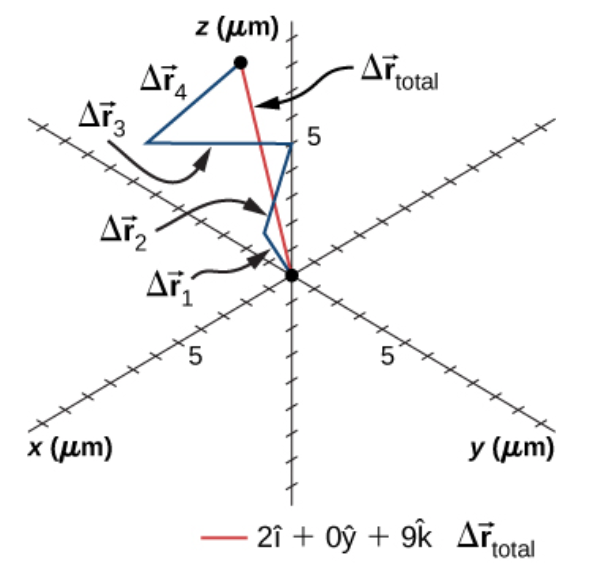
\includegraphics[width=0.6\textwidth,trim=0cm 2cm 0cm 0cm,clip=true]{figures/Brownian.png}
\caption{\label{fig:brown} An example of a displacement vector at different moments in time.}
\end{figure}
\end{frame}

\begin{frame}{Vectors as functions of time}
The particle in Fig. \ref{fig:brown} has four displacement vectors at four moments in time:
\begin{itemize}
\item $\vec{r}_{\rm 1} = 2.0\hat{i} + 1.0\hat{j} + 3.0\hat{k}\quad(\mu m)$ at $t_{\rm 1}$
\item $\vec{r}_{\rm 2} = -1.0\hat{i} + 0.0\hat{j} + 3.0\hat{k}\quad(\mu m)$ at $t_{\rm 2}$
\item $\vec{r}_{\rm 3} = 4.0\hat{i} + -2.0\hat{j} + 1.0\hat{k}\quad(\mu m)$ at $t_{\rm 3}$
\item $\vec{r}_{\rm 4} = -3.0\hat{i} + 1.0\hat{j} + 2.0\hat{k}\quad(\mu m)$ at $t_{\rm 4}$
\end{itemize}
What is the total displacement of the particle from the origin?
\end{frame}

\begin{frame}{Vectors as functions of time}
We can think of this type of problem as an accounting problem, lining up columns (units: $\mu m$):
\begin{figure}
\begin{tabular}{| c | c | c | c | c |}
\hline
$t_{\rm i}$ & $\vec{r}_{\rm i}(t_{\rm i})$ & $x(t_{\rm i})$ & $y(t_{\rm i})$ & $y(t_{\rm i})$ \\
\hline
$t_{\rm 1}$ & $\vec{r}_{\rm 1}(t_{\rm 1})$ & 2.0 & 1.0 & 3.0 \\
\hline
$t_{\rm 2}$ & $\vec{r}_{\rm 2}(t_{\rm 2})$ & -1.0 & 0.0 & 3.0 \\
\hline
$t_{\rm 3}$ & $\vec{r}_{\rm 3}(t_{\rm 3})$ & 4.0 & -2.0 & 1.0 \\
\hline
$t_{\rm 4}$ & $\vec{r}_{\rm 4}(t_{\rm 4})$ & -3.0 & 1.0 & 2.0 \\
\hline
\hline
$t_{\rm total}$ & $\vec{r}_{\rm total}(t_{\rm total})$ & 2.0 & 0.0 & 9.0 \\
\hline
\end{tabular}
\caption{\label{tab:account} Accounting for the different displacement components, in units of $\mu m$.}
\end{figure}
\end{frame}

\begin{frame}{Vectors as functions of time}
\begin{figure}
\centering
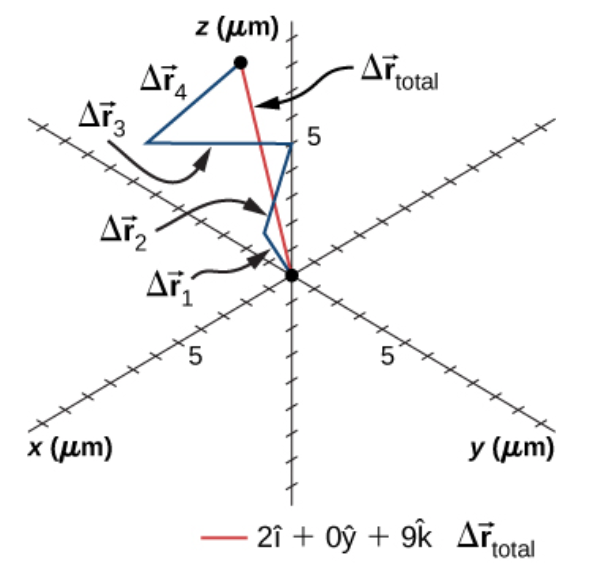
\includegraphics[width=0.6\textwidth]{figures/Brownian.png}
\caption{\label{fig:brown2} The total displacement of the particle is $\vec{r}_{\rm total} = 2.0\hat{i} + 0.0\hat{k} + 9.0\hat{k}\quad (\mu m)$.}
\end{figure}
\end{frame}

\begin{frame}{Vectors as functions of time}
\small
The 18th hole at Pebble Beach Golf Course is a dogleg to the left of length 496.0 meters.  The fairway off the tee is taken to be the x direction.  A golfer hits his tee shot a distance of 300 meters, corresponding to a displacement of $\vec{r}_{\rm 1} = 300.0 \hat{i} \quad (m)$, and then hits a second shot 189.0 meters with $\vec{r}_{\rm 2} = 172.0 \hat{i} + 80.3 \hat{j} \quad m$.  What is the final displacement from the tee?
\begin{itemize}
\item A: $\vec{r}_{\rm final} = 172.0 \hat{i} + 80.3\hat{j}\quad (m)$
\item B: $\vec{r}_{\rm final} = 172.0 \hat{i} + 380.3\hat{j}\quad (m)$
\item C: $\vec{r}_{\rm final} = 472.0 \hat{i} + 0.0\hat{j}\quad (m)$
\item D: $\vec{r}_{\rm final} = 472.0 \hat{i} + 80.3\hat{j}\quad (m)$
\end{itemize}
\end{frame}

\begin{frame}{Vectors as functions of time}
\small
If the first shot takes 5.0 seconds, the second shot takes 4.0 seconds, and the walking time in between the shots is 60.0 seconds, what is the average velocity vector for the ball after the two shots?
\begin{itemize}
\item A: $\vec{r}_{\rm final} = 1.7 \hat{i} + 8.3\hat{j}\quad (m/s)$
\item B: $\vec{v}_{\rm final} = 172.0 \hat{i} + 80.3\hat{j}\quad (m/s)$
\item C: $\vec{v}_{\rm final} = 6.8 \hat{i} + 1.2\hat{j}\quad (m)$
\item D: $\vec{v}_{\rm final} = 6.8 \hat{i} + 1.2\hat{j}\quad (m/s)$
\end{itemize}
\end{frame}

\begin{frame}{Vectors as functions of time}
The prior problem indicates something you may already have guessed:
\begin{equation}
\vec{v}_{\rm avg}(t) = v_{\rm x}(t) \hat{i} + v_{\rm y}(t) \hat{j} + v_{\rm z}(t) \hat{k} = \frac{\Delta\vec{r}}{\Delta t}
\label{eq:vel}
\end{equation}
\begin{itemize}
\item $v_{\rm x}(t)$ is the avg. velocity in the x-direction
\item $v_{\rm y}(t)$ is the avg. velocity in the y-direction
\item $v_{\rm z}(t)$ is the avg. velocity in the z-direction
\end{itemize}
In other words, we divide each displacement component by the time, to get a vector where each component is the average velocity in that direction.  $\Delta\vec{r} = \vec{r}_{\rm f} - \vec{r}_{\rm i}$.
\end{frame}

\begin{frame}{Vectors as functions of time}
Instantaneously, Eq. \ref{eq:vel} is true, if we \alert{take the limit} $\Delta t \to 0$:
\begin{equation}
\vec{v}(t) = \lim_{\Delta t \to 0} \frac{\Delta\vec{r}}{\Delta t} = \frac{dx}{dt}\hat{i} + \frac{dy}{dt}\hat{j} + \frac{dz}{dt}\hat{k}
\label{eq:vel2}
\end{equation}
\begin{itemize}
\item $\frac{dx}{dt}$ is the instantaneous velocity in the x-direction
\item $\frac{dy}{dt}$ is the instantaneous velocity in the y-direction
\item $\frac{dz}{dt}$ is the instantaneous velocity in the z-direction
\end{itemize}
\end{frame}

\begin{frame}{Vectors as functions of time}
The position of a particle is $\vec{r}(t) = 4.0t^2\hat{i} - 3.0 \hat{j} + 2.0t^2\hat{k}$ (m).  What is the velocity vector at $t=2$ seconds?  What is the average velocity between $t=0$ and $t=2$ seconds?
\begin{itemize}
\item A: $16\hat{x} + 8\hat{z}$ (m/s), $8\hat{x} + 4\hat{z}$ (m/s)
\item B: $8\hat{x} + 4\hat{z}$ (m/s), $4\hat{x} + 2\hat{z}$ (m/s)
\item C: $8\hat{x} + 8\hat{z}$ (m/s), $4\hat{x} + 4\hat{z}$ (m/s)
\item D: $4\hat{x} + 2\hat{z}$ (m/s), $4\hat{x} + 2\hat{z}$ (m/s)
\end{itemize}
\end{frame}

\begin{frame}{Vectors as functions of time}
Instantaneously, from Eq. \ref{eq:vel2}: 
\begin{equation}
\vec{a}(t) = \lim_{\Delta t \to 0} \frac{\Delta\vec{v}}{\Delta t} = \frac{dv_{\rm x}}{dt}\hat{i} + \frac{dv_{\rm y}}{dt}\hat{j} + \frac{dv_{\rm z}}{dt}\hat{k}
\label{eq:vel3}
\end{equation}
\begin{itemize}
\item $\frac{dv_{\rm x}}{dt}$ is the instantaneous acceleration in the x-direction
\item $\frac{dv_{\rm y}}{dt}$ is the instantaneous acceleration in the y-direction
\item $\frac{dv_{\rm z}}{dt}$ is the instantaneous acceleration in the z-direction
\end{itemize}
\end{frame}

\begin{frame}{Vectors as functions of time}
The velocity of a particle is $\vec{v}(t) = 8.0t\hat{i} + 4.0t\hat{k}$ (m/s).  What is the acceleration vector at $t=2$ seconds?  What is the average acceleration between $t=0$ and $t=2$ seconds?
\begin{itemize}
\item A: $4\hat{i} + 4\hat{k}$ (m/s$^2$), $2\hat{i} + 2\hat{k}$ (m/s$^2$)
\item B: $8\hat{i} + 4\hat{k}$ (m/s$^2$), $8\hat{i} + 4\hat{k}$ (m/s$^2$)
\item C: $8\hat{i} + 8\hat{k}$ (m/s$^2$), $4\hat{i} + 4\hat{k}$ (m/s$^2$)
\item D: $4\hat{i} + 8\hat{k}$ (m/s$^2$), $2\hat{i} + 4\hat{k}$ (m/s$^2$)
\end{itemize}
\end{frame}

\begin{frame}{Vectors as functions of time}
\small
The displacement of a particle is $\vec{x}(t) = (2t+3)\hat{i}+(\frac{3}{2}t^2+2t+3.0)\hat{j}$ (m).  What is the horizontal velocity (the $\hat{i}$-component of the velocity) at $t=4$ seconds?  At $t=10$ seconds?
\begin{itemize}
\item A: 4 m/s, 4 m/s
\item B: 2 m/s, 4 m/s
\item C: 2 m/s, 2 m/s
\item D: 4 m/s, 2 m/s
\end{itemize}
\end{frame}

\begin{frame}{Vectors as functions of time}
\small
The displacement of a particle is $\vec{x}(t) = (2t+3)\hat{i}+(\frac{3}{2}t^2+2t+3.0)\hat{j}$ (m).  What is the vertical velocity (the $\hat{j}$-component of the velocity) at $t=4$ seconds?  At $t=10$ seconds?
\begin{itemize}
\item A: 14 m/s, 32 m/s
\item B: 32 m/s, 14 m/s
\item C: 12 m/s, 30 m/s
\item D: 30 m/s, 12 m/s
\end{itemize}
\end{frame}

\begin{frame}{Vectors as functions of time}
Notice in the previous example, the x-velocity and y-velocity were not the same function. \\
\vspace{0.5cm}
In the kinematic description of motion, \alert{\textit{we are able to treat the different components of motion separately.}}  In many cases, motion in the horizontal direction does not affect motion in the vertical direction, and vice versa.\\
\vspace{0.5cm}
\small
\framebox[1.1\width]{\textbf{Motions in displacement components are independent.}} \\
\vspace{1cm}
\textit{(Exception: non-conservative forces.  More on this later.)}
\end{frame}

\section{Combining free-fall and vector components: projectile motion}

\begin{frame}{Projectile motion}
\small
\begin{figure}
\centering
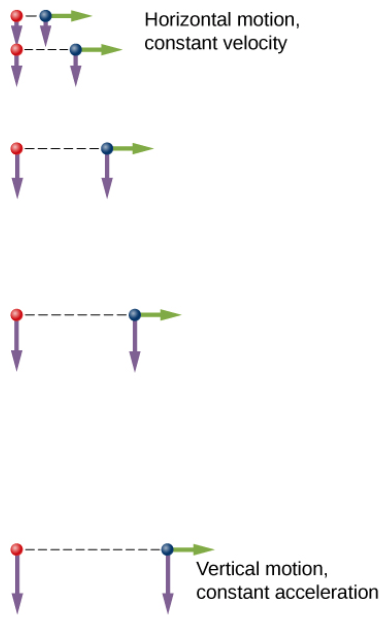
\includegraphics[width=0.35\textwidth]{figures/fall.png}
\caption{\label{fig:fall} The red particle accelerates vertically, with no horizontal velocity.  The blue particle acclerates vertically, with some horizontal velocity.}
\end{figure}
\end{frame}

\section{Lab Activity}

\begin{frame}{Projectile motion}
Is this true?  Figure \ref{fig:fall} is testable by experiment. \\
\vspace{0.5cm}
\small
Procedure:
\begin{enumerate}
\item Obtain two marbles, a meter stick, and a stopwatch.
\item Measure the height of the lab bench, $\Delta x$.
\item We are going to drop a marble from this height ($\Delta x$) and record the time.  Show first algebraically that the predicted time for the marble to fall is $t = \sqrt{2\Delta x/g}$.
\item Measure $t$ for several trials.  Does it match the expected result $\sqrt{2\Delta x/g}$?  What are sources of error?
\item Repeat the measurement, but \textbf{roll the marble off of the table instead of dropping it} from $\Delta x$.  Does the average result for $t$ change?
\end{enumerate}
\end{frame}

\begin{frame}{Projectile motion}
\small
We now have learned that (a) motions in displacement components are \textit{independent}, and (b) when acceleration is in \alert{one direction} (vertical) only, the motion is \textit{projectile motion}.  Our usual equations of motion for no acceleration (horizontal), and constant acceleration (vertical) apply \textit{independently}:
\begin{columns}[T]
\begin{column}{0.5\textwidth}
\begin{align}
y(t) &= y_{\rm 0} + v_{\rm 0,y} t - \frac{1}{2}gt^2 \label{eq:main1} \\
v_{\rm y}(t) &= -gt+v_{\rm 0,y} \label{eq:main2} \\
v_{\rm y}^2 &= v_{\rm y,0}^2 - 2g(y-y_{\rm 0}) \label{eq:main3}
\end{align}
\end{column}
\begin{column}{0.5\textwidth}
\begin{align}
x(t) &= x_{\rm 0} + v_{\rm 0,x}t \label{eq:main4} \\
v_{\rm x}(t) &= v_{\rm 0,x} \label{eq:main5}
\end{align}
\end{column}
\end{columns}
\end{frame}

\begin{frame}{Projectile Motion}
\small
Projectile motion is a good topic to introduce the concept of \textit{boundary conditions}.  The \textit{physics} of projectile motion is the same for all situations, but the \textit{individual cases and numbers} might not be the same. \\
\vspace{0.5cm}
Suppose we are given the initial velocity and angle of a object that undergoes projectile motion.  To use Eqs. \ref{eq:main1}-\ref{eq:main5}, we need $v_{\rm 0,x}$ and $v_{\rm 0,y}$, the initial horizontal and vertical velocity components, respectively.
\end{frame}

\begin{frame}{Projectile Motion}
\small
Suppose we are given the initial velocity and angle of a object that undergoes projectile motion.  To use Eqs. \ref{eq:main1}-\ref{eq:main5}, we need $v_{\rm 0,x}$ and $v_{\rm 0,y}$, the initial horizontal and vertical velocity components, respectively.\\
\begin{figure}
\centering
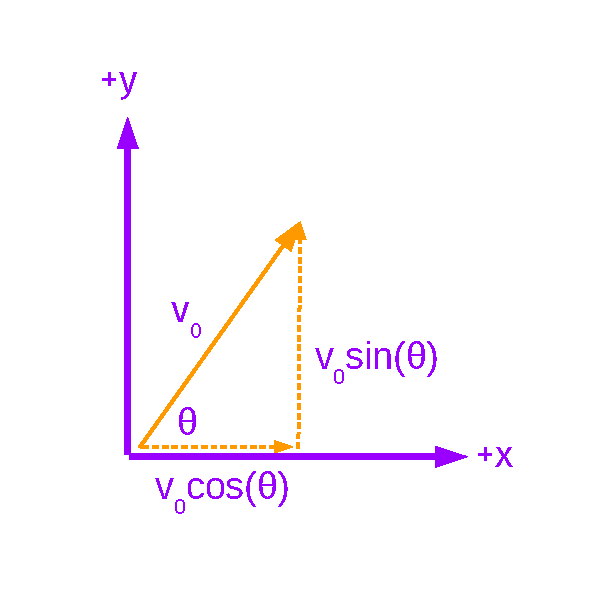
\includegraphics[width=0.5\textwidth,trim=1cm 1cm 1cm 1cm,clip=true]{figures/Vectors1.pdf}
\caption{\label{fig:components} The initial velocity $v_{\rm 0}$ is broken into components.}
\end{figure}
\end{frame}

\begin{frame}{Projectile Motion}
\small
During a fireworks display, a shell is shot into the air with an initial speed of 50 m/s, at an angle of 60$^{\circ}$ above horizontal.  The fuse is timed to ignite the shell just as it reaches its highest point above the ground.  Calculate the height at which the shell explodes.
\begin{itemize}
\item A: 190 m
\item B: 100 m
\item C: 110 m
\item D: 250 m
\end{itemize}
\end{frame}

\begin{frame}{Projectile Motion}
\small
How much time passes between the launch and the explosion?
\begin{itemize}
\item A: 3.9 seconds
\item B: 4.3 seconds
\item C: 5.1 seconds
\item D: 10.0 seconds
\end{itemize}
\end{frame}

\begin{frame}{Projectile Motion}
What is the horizontal displacement of the shell when it explodes?
\begin{itemize}
\item A: 108 meters
\item B: 98 meters
\item C: 98 degrees
\item D: 150 meters
\end{itemize}
\end{frame}

\begin{frame}{Projectile Motion}
\small
Let's try gaining visual intuition about projectile motion through the following program: \\
\vspace{0.25cm}
\url{http://galileoandeinstein.physics.virginia.edu/more_stuff/Applets/Projectile/projectile.html}\\
\begin{enumerate}
\item First, set air resistance to zero, at bottom right.
\item Make ten measurements of $g$ by creating some projectile trajectories, and taking the ratio $g = v_{\rm 0,y}^2/(2\Delta y)$.  What value do you obtain, on average?
\item Now, set air resistance to $b/m \approx 0.02$, and repeat the ten measurements.  What value do you obtain?
\item Explain why this value is smaller, larger, or equal to the first set of measurements.
\end{enumerate}
\end{frame}

\begin{frame}{Projectile Motion}
Projectile motion in two dimensions, with constant acceleration in one dimension, produces \textit{quadratic curves}.  How do we obtain the \alert{trajectory}, or $y(x)$ for these curves?  Looking at the x-direction:\\
\begin{align}
x &= v_{\rm 0}\cos(\theta) t \\
t &= \frac{x}{v_{\rm 0} \cos(\theta)} \label{eq:subst}
\end{align}
\end{frame}

\begin{frame}{Projectile Motion}
Substituting in Eq. \ref{eq:subst} for $t$ into the equation for vertical displacement gives:\\
\begin{align}
y(t) - y_{\rm 0} &= -\frac{1}{2}g\frac{x^2}{v_{\rm 0}^2\cos^2(\theta)} + \tan(\theta) x \\
y(t) - y_{\rm 0} &= -\left(\frac{g}{2v_{\rm 0}^2\cos^2(\theta)}\right)x^2 + \tan(\theta) x \\
y(x) - y_{\rm 0} &= -\left(\frac{g}{2v_{\rm 0}^2\cos^2(\theta)}\right)x^2 + \tan(\theta) x \label{eq:projfinal}
\end{align}
In Eq. \ref{eq:projfinal}, we are simply saying that $y(x)$ is some quadratic.  (It's still true that $y$ and $x$ are both functions of \textit{time}, however, those functions of time are related).
\end{frame}

\begin{frame}{Projectile Motion}
A space explorer is on a moon around another planet, and wants to measure $g$.  She tosses a pebble from an initial height of 2 meter, at an angle of 45 degrees above horizontal, with an initial velocity of 2 m/s.  When it lands, the horizontal displacement is 10 meters.  What is the gravitational acceleration $g$?
\begin{itemize}
\item A: 0.125 m/s$^2$
\item B: 0.25 m/s$^2$
\item C: 0.5 m/s$^2$
\item D: 1.0 m/s$^2$
\end{itemize}
\end{frame}

\begin{frame}{Projectile Motion}
Other useful equations are for the \textit{time-of-flight}, and the \textit{range}, concepts we've already seen in several examples: \\
\begin{align}
T_{\rm tof} &= \frac{2v_{\rm 0}\sin\theta}{g} \\
R &= \frac{v_{\rm 0}^2\sin2\theta}{g}
\end{align}
\end{frame}

\begin{frame}{Projectile Motion}
\alert{Algebraic challenge}: Show that the ratio of the range to the time is just the horizontal velocity, using the trigonometric identity $\sin(2\theta) = 2\sin\theta\cos\theta$.
\end{frame}

\section{Relative Motion and Reference Frames}

\begin{frame}{Relative Motion and Reference Frames}
Thus far, we have been discussing \textit{kinematics} with respect to a \textit{fixed frame of reference}.  Usually, we think of this frame of reference as the Earth.  If we kick a soccer ball, we know how to use equations to describe the motion.  What if we are moving, and the ball is moving with us, when we kick it?
\end{frame}

\begin{frame}{Relative Motion and Reference Frames}
Michael is running at 5 m/s, with a soccer ball rolling with him at the same speed.  He shoots the ball, such that he judges the speed to be 10 m/s.  What is the speed of the ball for someone who is observing, and standing still?
\begin{itemize}
\item A: 5 m/s
\item B: 10 m/s
\item C: 15 m/s
\item D: Cannot determine.
\end{itemize}
\end{frame}

\begin{frame}{Relative Motion and Reference Frames}
So we see that relative motion is about adding and subtracting vectors.  Let's introduce a notation so that we always add vectors from reference frames correctly.  If two frames of reference (think of them as moving coordinate systems) $S$ and $S'$ are both moving with respect to each other.  The position of a particle $P$ in frame $S$ is \\
\begin{equation}
\vec{r}_{\rm PS} = \vec{r}_{\rm PS'} + \vec{r}_{\rm S'S}
\end{equation}
\end{frame}

\begin{frame}{Relative Motion and Reference Frames}
\small
\begin{equation}
\vec{r}_{\rm PS} = \vec{r}_{\rm PS'} + \vec{r}_{\rm S'S}
\end{equation}
\begin{figure}
\centering
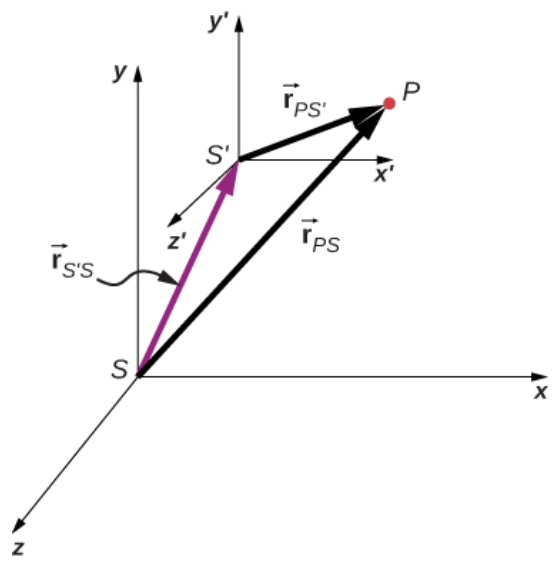
\includegraphics[width=0.45\textwidth]{figures/frames.png}
\caption{\label{fig:frame} \small ``To get where you are going, first you must know where you are.''}
\end{figure}
\end{frame}

\begin{frame}{Relative Motion and Reference Frames}
For positions:
\begin{equation}
\vec{r}_{\rm PS} = \vec{r}_{\rm PS'} + \vec{r}_{\rm S'S}
\end{equation}\\
Since velocities are just the time-derivatives of positions:
\begin{equation}
\vec{v}_{\rm PS} = \vec{v}_{\rm PS'} + \vec{v}_{\rm S'S}
\end{equation}\\
...and accelerations are just the time-derivatives of velocities:
\begin{equation}
\vec{a}_{\rm PS} = \vec{a}_{\rm PS'} + \vec{a}_{\rm S'S}
\end{equation}
\end{frame}

\section{Answers}

\begin{frame}{Answers}
\begin{columns}[T]
\begin{column}{0.5\textwidth}
\begin{itemize}
\item To the right, positive
\item At the peak height, yes, yes
\item $\vec{r}_{\rm final} = 472.0 \hat{i} + 80.3\hat{j}\quad (m)$
\item $\vec{v}_{\rm final} = 6.8 \hat{i} + 1.2\hat{j}\quad (m/s)$
\item $16 \hat{x} + 8\hat{z}$ (m/s), $8\hat{x} + 4\hat{z}$ (m/s)
\item $8\hat{i} + 4\hat{k}$ (m/s$^2$), $8\hat{i} + 4\hat{k}$ (m/s$^2$)
\item 2 m/s, 2 m/s
\item 14 m/s, 32 m/s
\item 190 m
\end{itemize}
\end{column}
\begin{column}{0.5\textwidth}
\begin{itemize}
\item 4.3 seconds
\item 108 meters
\item 0.5 m/s$^2$
\item $R/T = v_{\rm 0} \cos\theta = v_{\rm x,0}$
\end{itemize}
\end{column}
\end{columns}
\end{frame}

\end{document}
